\section{Eindproduct}
Het doel van de afstudeer opdracht is het maken van een proof of concept versie van een nieuw CMS.
Hierbij was bepaald om de CMS UI weg te laten om de scope van de opdracht realisitisch te houden.
Er is wel gebruik gemaakt van een developer interface genaamd swagger \parencite{Swagger}.
Swagger is een software oplossing dat een UI geeft aan een API zodat er makkelijker mee geinteracteerd kan worden.
In figuur \ref{fig:SwaggerApi} is de swagger UI te zien van de CMS API.

\whitespace
\begin{graphic}
    \captionsetup{type=figure}
    \caption{Swagger interface}
    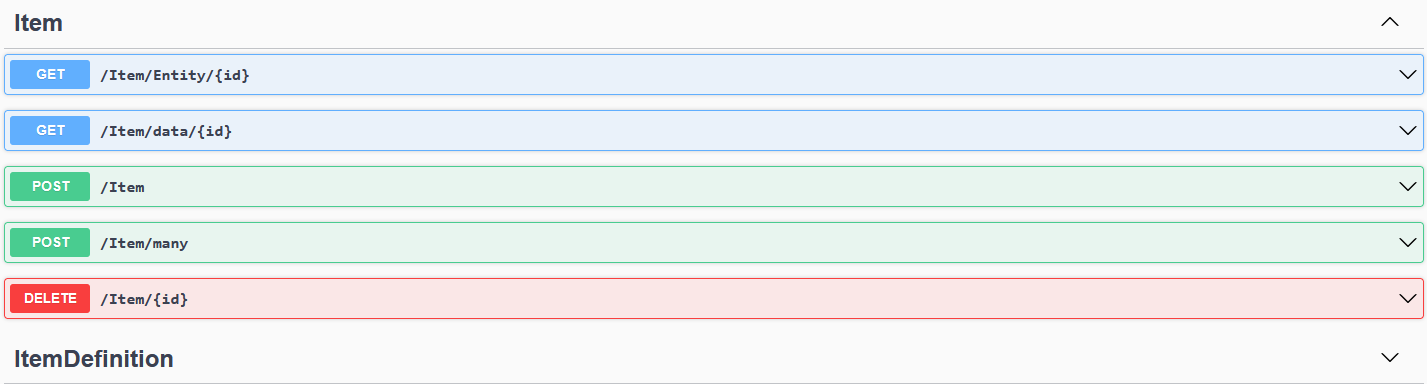
\includegraphics[scale=0.4]{SwaggerUI.png}
    \label{fig:SwaggerApi}
\end{graphic}

\subsection{Implementatie Datamodel}
Het ontwerp dat is gemaakt, mist een specifieke implementatie voor het gegevenstype \qw{content}, zoals te zien is in figuur \ref{fig:ClassDiagramItemFieldWithDefinition} (raadpleeg sectie \ref{subsection:Datamodel} voor meer details).
Dit gegevenstype zou verschillende vormen van gegevens moeten kunnen bevatten, zoals strings, getallen en booleans.
In programmeertalen zoals Python en JavaScript is dit geen probleem, omdat ze dynamisch getypeerd zijn.
Dit betekent dat het gegevenstype van variabelen niet van tevoren gespecificeerd hoeft te worden.
Een van de randvoorwaarden is dat het afstudeerproduct in C \# wat een statisch getypeerde taal.
% Echter, het afstudeerproject moet worden gerealiseerd in een statisch getypeerde taal (C\#).

\whitespace
Dit is opgelost door gebruik te maken van een abstracte superklassen \textit{FieldValueBase}.
Deze superklasse heeft verschillende implementaties die de verschillende datatypes kunnen onderstuenen.
Een klasse diagram hiervan is te zien in figuur \ref{fig:ImplementatieFields}.
In het klassediagram is er één implementatie getoond van \textit{FieldValueBase} om het voorbeeld simpel te houden.

\whitespace
\begin{graphic}
    \captionsetup{type=figure}
    \caption{Implementaite Fields}
    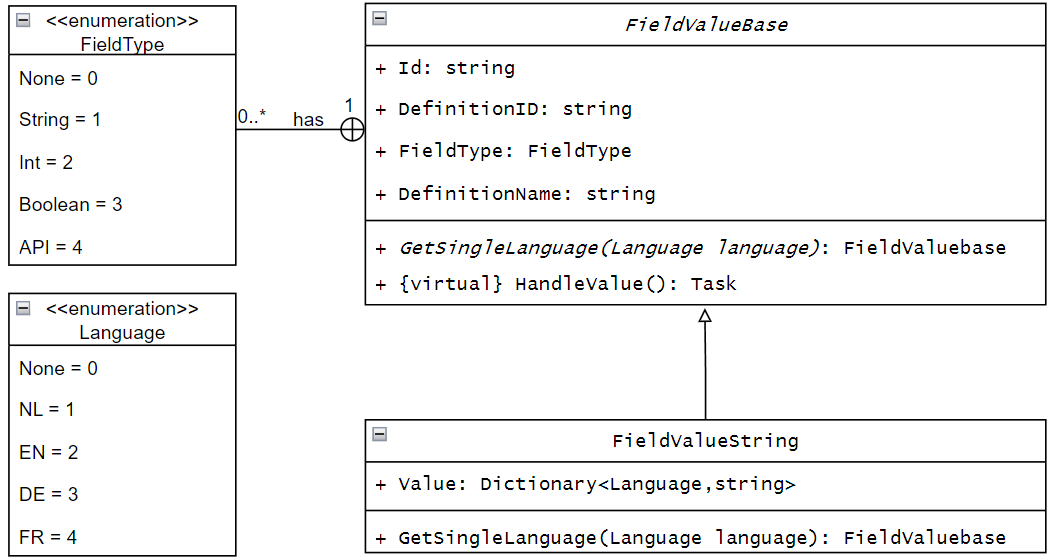
\includegraphics[scale=0.4]{FieldImplementation.png}
    \label{fig:ImplementatieFields}
\end{graphic}

\whitespace
Een van de kenmerken van \textit{FieldValueString} is dat de data wordt opgeslagen in een dictionary met de taal als key.
De huidige aanpak van het CMS voor meertaligheid houdt in dat een kopie van de originele site wordt gemaakt en vervolgens wordt vertaald.
Door vertalingen op te slaan in de \textit{fields}, kunnen vertalingen eenvoudig worden toegevoegd.
Dit resulteert in het onderhouden van slechts één site in plaats van een aparte site voor elke taal.

\whitespace
Het nadeel van een abstracte klasse als datatype gebruiken is dat de standaard C\# oplossing van \textit{Json Deserialisation} niet goed werkt.
Het probleem ligt in het interpreteren van de abstracte types naar de concrete implementaties.
Hierdoor kunnen controller enpoints niet de json data verwerken omdat er niet gedeserialiseerd mag worden van een abstracte klas.
Hierom wordt er gebruik gemaakt van een .NET 8 oplossing genaamd \textit{Model binders}.
Model binders zorgen ervoor dat controllers direct met het model kunnen werken in plaats van het HTTP request \parencite{ModelBinders}.
De geïmplementeerde versie van de model binder is te zien in figuur \ref{fig:Modelbinder}.
Verder zijn de mappers te zien die gebruikt worden in figuur \ref{fig:ModelbinderMappers}.

\whitespace
\begin{graphic}
    \captionsetup{type=figure}
    \caption{Item Modelbinder}
    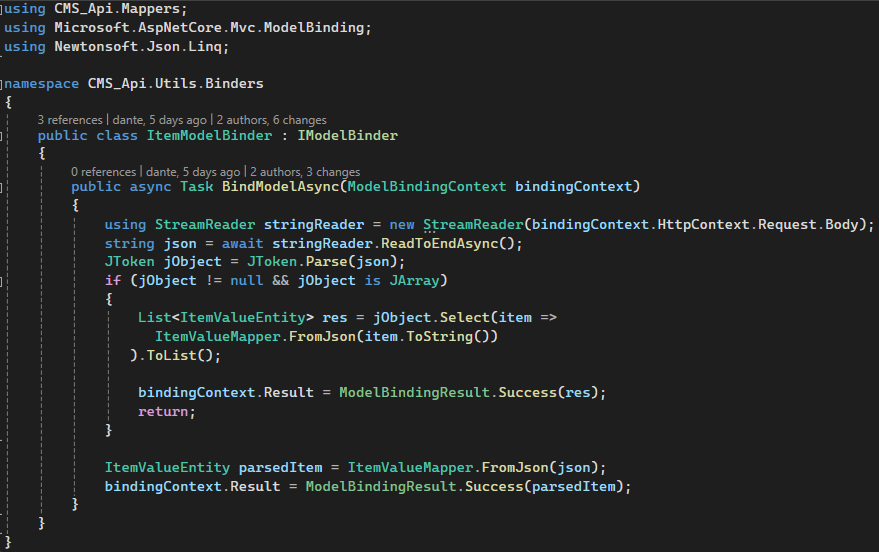
\includegraphics[scale=0.5]{ImplementatieModelBinder.png}
    \label{fig:Modelbinder}
\end{graphic}

\whitespace
\begin{graphic}
    \captionsetup{type=figure}
    \caption{Gebruikte mappers voor de modelbinder}
    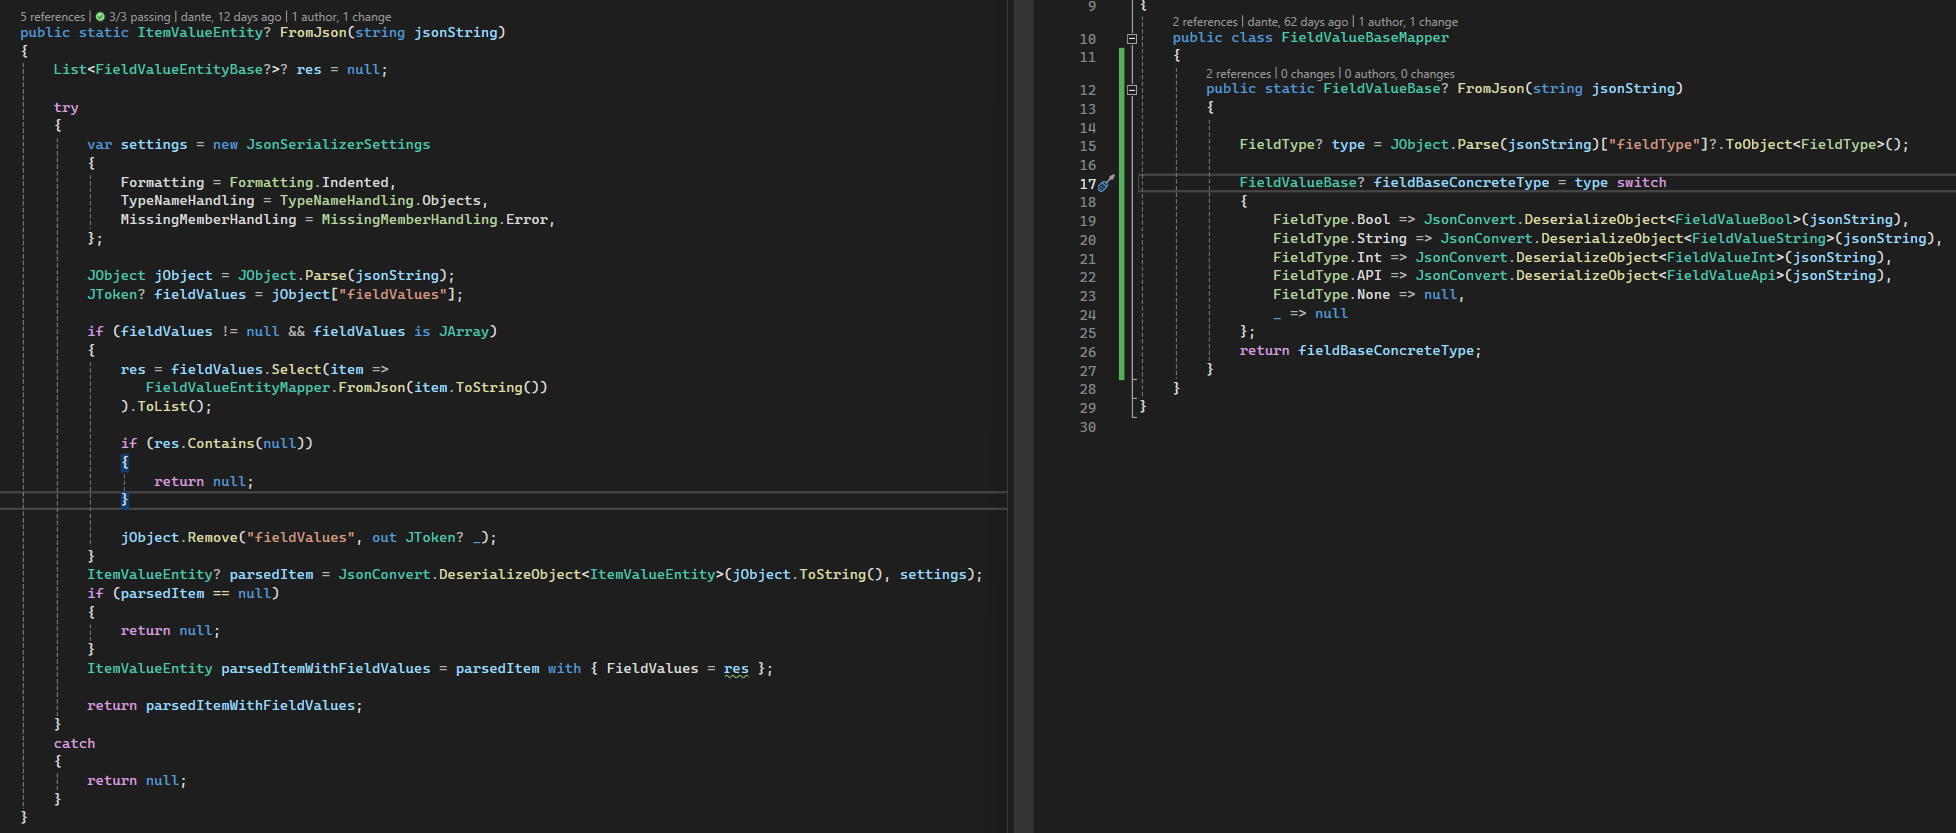
\includegraphics[scale=0.34]{implementatieModelBinderMappers.png}
    \label{fig:ModelbinderMappers}
\end{graphic}

\subsection{Implementatie Frontend}
Het laatste deel van de afstudeer applicatie is de \gls{Beheerder} zijn website.
Deze website moet de data van de CMS-API kunnen renderen.
Er is gekozen om een site na te bouwen, de site die hiervoor gekozen is de Snakeware site (Snakeware.com).
Dit is gedaan omdat de developers van de site makkelijk aangesproken kunnen worden voor mogelijke ondersteuning.
Verder is de repository beschikbaar gesteld zodat verschillende stijlingen overgenomen kunnen worden.

\whitespace
Om dit te realiseren is het ontwerp uitgewerkt voor de frontend (zie sectie \ref{sec:FrontendProcessView}).
Het eerste type is de simpelste variant van de frontend onderdelen. 
Het voorbeeld dat gebruikt is rendered een stuk tekst met een titel en optioneel een button.

\whitespace
Dit wordt gedaan door de verschillende \textit{fields} te gebruiken en hiermee de variabelen te vullen.
Deze variabelen worden vervolgens gebruikt in het component om het te renderen op de site.
De implementatie hiervan is te zien in figuur \ref{fig:FrontendImplementatieComponent}.
Verder is er ook te zien dat de \qw{Link} field gebruikt wordt om  een redirect uit te voeren zodra er opgeklikt wordt.

\whitespace
\begin{graphic}
    \captionsetup{type=figure}
    \caption{Implemenatie van Vue component}
    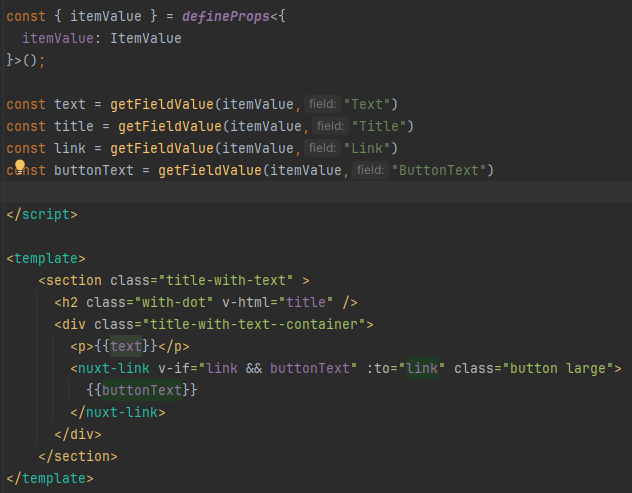
\includegraphics[scale=0.8]{ImplementationOfComponentVue.png}
    \label{fig:FrontendImplementatieComponent}
\end{graphic}

\whitespace
Het tweede type component is een Container component die te zien is in figuur \ref{fig:FrontendContainerImplementatie}.
Dit component rendered alle \qw{implementatie componenten} dit wordt gedaan door gebruik te maken van het component \qw{component}.
Het \qw{component} component wordt ook wel v-component genoemd om de verwarringen te voorkomen.
Dit v-component kan gerenderd worden als elk component dat je mee geeft.
Hierdoor is het makkelijk om op run time te bepalen welk component gerenderd moet worden.
Verder wordt het Container zelf ook gebruikt als het item geen fields heeft.
Hierdoor kan de content recursief gerenderd worden.

\newpage

\whitespace
\begin{graphic}
    \captionsetup{type=figure}
    \caption{Implementatie container component}
    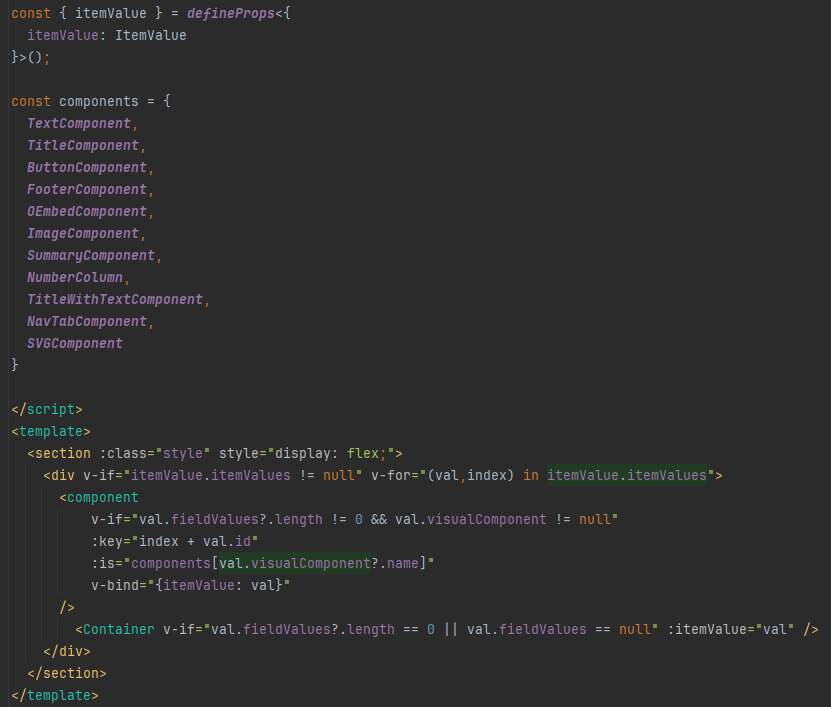
\includegraphics[scale=0.5]{ImplementatieContainersVue.png}
    \label{fig:FrontendContainerImplementatie}
\end{graphic}

\whitespace
Door het gebruik te maken van deze 2 type componenten is het mogelijk om de snekware site te renderen.
De volledige rendering van de site is te zien in figuur \ref{fig:Frontend}.

\whitespace
\begin{graphic}
    \captionsetup{type=figure}
    \caption{Frontend}
    
\includegraphics[scale=0.3]{Placeholder.jpg}
    \label{fig:Frontend}
\end{graphic}

\todo[inline]{Wil ik als laatste doen}


